%!TEX root = /Users/zolkko/Projects/zolkko-alarm/doc/main.tex
\section{Выбор инструментальных средств разработки микроконтроллерного программно-аппаратного комплекса}

\subsection{Выбор микроконтроллера}
Основными требованиями предъявляемыми мной к центральному вычислительному устройству
создаваемого устройства является:
\begin{itemize}
	\item{} невысокая стоимость;
	\item{} низкое энергопотребление;
	\item{} в число поддерживаемой переферии должен присутствовать ЦАП;
	\item{} аппаратная поддержка SPI;
	\item{} поддержка производителем этого рода устройств;
	\item{} доступность устройства;
	\item{} <<сильное>> сообщество разработчиков под эту архитектуру;
	\item{} наличие литературы и справочных материалов.
\end{itemize}


По всем этм пунктам идеально подходит микроконтрллер семейства XMega компании ATmel -- atxmega32a4.
Этот микроконтроллер полностью отвечает минимальным требованиям. В целях достижения максимальной
производительности и параллелизма у микроконтроллеров AVR используется
Гарвардская\\*
архитектура (рисунок \ref{img:avr_arch}) с отдельными памятью и шинами программ и данных. Инструкции,
хранящиеся в памяти программ, выполняются на одноуровневом конвейере. Это означает, что
во время выполнения одной инструкции выполняется предварительная выборка из памяти программ
следующей инструкции. Данная концепция делает возможным выполнение по одной инструкции за
каждый цикл синхронизации.

\begin{figure}[ht]
	\center{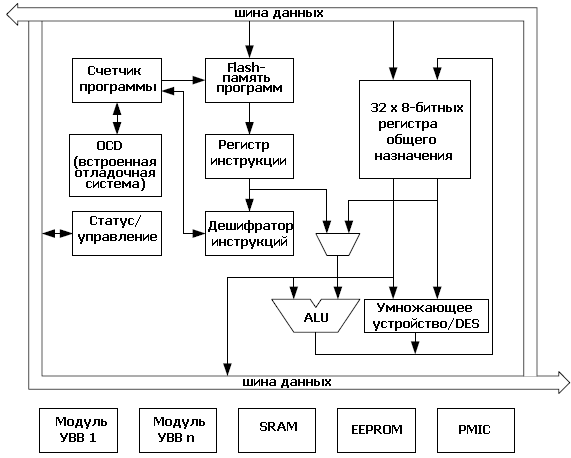
\includegraphics[bb=0 0 590 460, clip, scale=0.6]{avr_arch.png}}
	\caption{Архитектура AVR}
	\label{img:avr_arch}
\end{figure}


Так же в случае необходимости может быть заменён на более мощьный микроконтроллер того же семейства.
Для обеспечения этого функционала компания Atmel предприняла ряд шагов.

\begin{par}
    1. Была реорганизована область памяти, таким образом, чтобы все связанные между
            собой регистры располагались в памяти строго последовательно.
\end{par}
\begin{par}
    2. Была переписана стандартная библиотека C/C++, так чтобы обеспечивалась
            максимальная переносимость кода написанного для одного микроконтроллера
            на другой микроконтроллер того же семейства.
\end{par}

Микроконтроллеры серии XMega обладают следующими характеристиками:
\begin{itemize}
	\item{} 8/16-разрядное высокопроизводительное RISC ЦПУ AVR;
	\item{} 138 инструкций;
	\item{} аппаратное умножающее устройство;
	\item{} 32 8-битных регистра, напрямую подключенные к АЛУ
	\item{} прямая адресация до 16 Мбайт памяти программ и 16 Мбайт памяти данных;
	\item{} полная поддержка 16/24-битного доступа к 16/24-битным регистрам ввода-вывода;
	\item{} эффективная поддержка 8-, 16- и 32-битных арифметических инструкций;
	\item{} защита от изменения настроек критических функций системы.
\end{itemize}

Помимо этого, по сравнению с предыдущим семейством Mega \cite{avrref}, в микроконтроллеры семейства
XMega был внесен ряд значительных изменений.

\begin{par}
    1. Свехмалое энергопотребление обеспечиваемое технологией picoPower второго поколения.
    picoPower позволяет еще больше улучшить эффективность использования батарейного источника.
    То, что микроконтроллеры гарантируют нормальное функционирование при напряжении 1.6 В означает,
    что, например, в составе мобильных телефонов, они могут быть запитаны от стабилизированного
    источника напряжением 1.8В 10\%, тем самым, позволяя снизить себестоимость системы и увеличить
    длительность работы от батарейного источника. 
\end{par}

\begin{par}
    2. Event System -- позволяет организовать передачу данных между встроенными периферийными
    устройствами без вмешательства ЦПУ или использования ПДП.
    Этим гарантируется 100\% предсказуемость и малое время реагирования.
    До 8 одновременных событий или условий прерывания в периферийных устройствах могут автоматически
    инициировать действия в других периферийных устройствах \cite{avrxm}.
\end{par}

\begin{par}
    3. 12-разрядные АЦП и ЦАП. Для обеспечения высокоточной обработки аналоговых сигналов в состав 
    микроконтроллеров XMEGA интегрированы 12-битные преобразователи аналоговых сигналов. АЦП
    микроконтроллеров XMEGA могут достигать частоты преобразования до 2 МГц, что делает их самыми
	быстродействующими и точными на фоне АЦП обычных микроконтроллеров.
	Поскольку микроконтроллеры XMEGA также интегрируют два 12-битных ЦАП на частоту преобразования
	до 1 МГц и четыре усовершенствованных аналоговых компаратора, это делает их лидерами по
	степени интеграции компонентов для аналоговой обработки.
\end{par}

\begin{par}
   4. Расширена функциональность портов ввода-вывода общего назначения. Каждый из портов
    ввода-вывода может быть сконфигурирован как источник внешнего прерывания, при этом событие внешнего прерывания
    может минуюя ЦПУ запускать обработку данных используя модуль прямого доступа к памяти. \\*
    Новыми доступными состояниями портов ввода-вывода стали totem-pull, bus-keeper, wired-or, wired-and.
\end{par}


\subsection{Язык программирования микроконтроллера}
\begin{par}
Микропрограммы для микроконтроллеров XMega можно писать на нескольких языках программирования.
Сама компания Atmel предоставляет для программирования своих устройств два средства разработки:
	\begin{enumerate}
		\item{}AVR assembler -- язык низкого уровня, транслирует исходный код пользовательской
                программы в объектны и исполняемый код, его применение позволяет
                добиться от программы наибольшей производительности;
		\item{}AVR-GCC -- кодогенератор и набор дополнительных утилит для Gnu C Compiller от
                компании Atmel, активно поддерживаемый сообществом разработчиков, а так же
                входящий в комплект среды разработки AVR Studio, AVR32 Stdio и
                распростроняемый на правах свободного программного обеспечения, в состав
				которого входят компиляторы языка C и C++.
	\end{enumerate}
\end{par}

\begin{par}
В начале 2011 года компания предоставила новую версию своей интегрированной системы
разработки - AVR Studio 5. В отличии от предшественника, новая система позволяет разрабатывать
программное обеспечение для всех семейств микроконтроллеров AVR используюя единую среду разработки.
\end{par}

\begin{par}

\begin{figure}[ht]
	\center{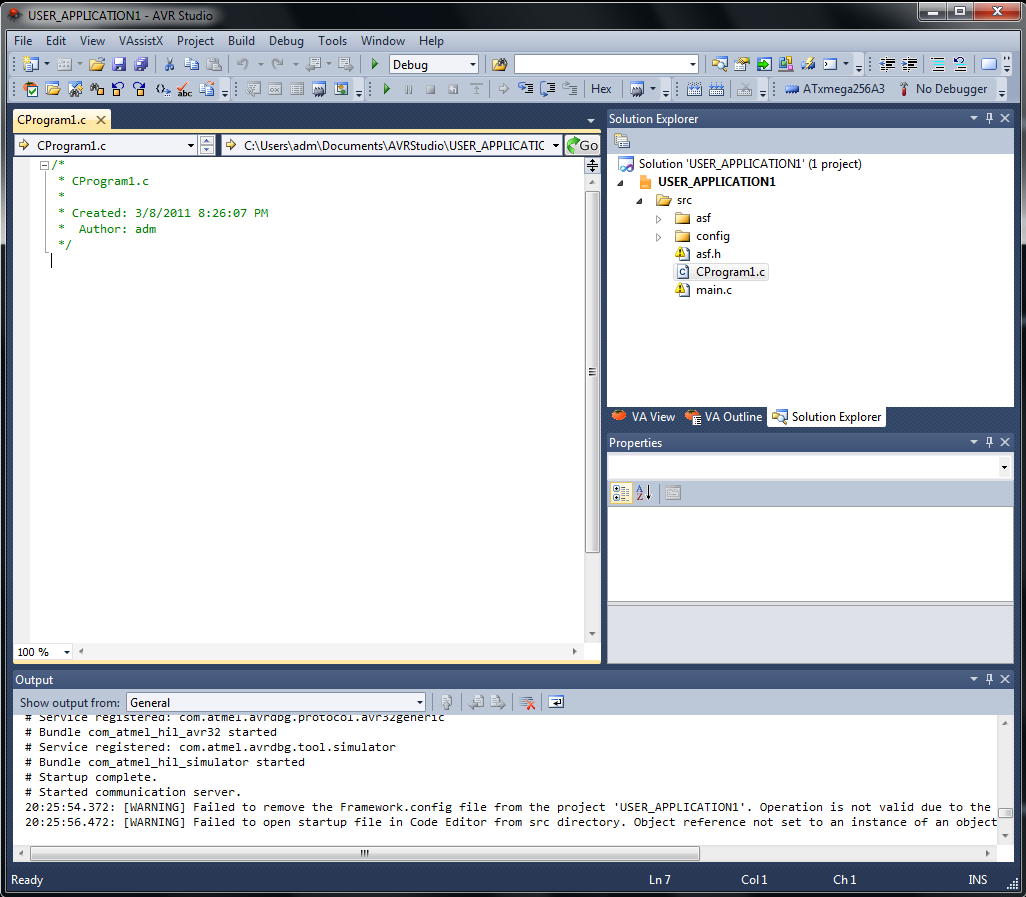
\includegraphics[bb=0 0 800 700, clip, scale=0.5]{avrstudio5.png}}
	\caption{AVR Studio 5}
	\label{img:avr_studio}
\end{figure}


Новая среда разработки AVR Studio 5 (рисунок \ref{img:avr_studio}) основана на базе лидирующего
продукта -- Microsoft Visual Studio.
И так же как и предшественники, новая версия AVR Studio 5  распространяется бесплатно.
В качестве компилятора и кодогенератора в AVR Studio 5 по прежнему используется AVR-GCC,
что позволяет продолжать использовать уже существующие наработки.
\end{par}

\begin{par}
Считается \cite{avrev}, что для разработки эффективного встраиваемого приложения для 8-битных микроконтрллеров
AVR наиболее целесообразно применять язык ассемблера или в случае, когда необходимо добиться
большей читаемости и поддерживаемости приложения -- язык С.
Однако, лидирующая группа японских производителей ЦПУ, возглавляемая NEC, Hitachi, Fujitsu и Toshiba,
разработала специализированных диалект языка C++ --- Embedded C++ (EC++), позволяющий применять
C++ для встраиваемых систем. Основная цель разработки --- перенос существующих методологий и шаблонов
программирования C++ в облать применения встраивамых систем.
При этом программы код генерируемых компиляторами EC++ может даже дать приемущества по сравлению
с языком C. Так как сама структура языка C++ позволяет минимизировать объём кода и одновременно
повышая его эффективность.
\end{par}

\begin{par}
Однако, при выборе в качестве языка программирования C++, из текущей реализации поставляемой с AVR-GCC,
необходимо учитывать некоторые её ограничения.
\end{par}

\begin{par}
 	1. В наборе компиляторов AVR-GCC отсутствует стандартная библиотека C++.
\end{par}

\begin{par}
	2. Необходимо помнить, что EC++ -- это только подмножество C++, по этому некоторые особенности языка были
        убраны из стандарта:
        \begin{itemize}
            \item{} множественное наследование;
            \item{} базовые виртульаные классы;
            \item{} информация времени исполнения;
            \item{} приведение типов (static\_cast, dynamic\_cast, reinterpret\_cast и const\_cast);
            \item{} квалификаторы типов;
            \item{} пространства имён;
            \item{} исключения;
            \item{} шаблоны.
        \end{itemize}
\end{par}



\subsection{Выбор языка программирования сетевого сервиса}

При проектировании сетевого сервиса от инструментального средства ожидается, чтобы оно
отвечало следующим требованиям \cite{technob}:

\begin{enumerate}
	\item{} инструментальное средство должно быть высокого уровня --- язык высокого уровня,
            освобождает разработчика от рутинной работы вроде ручного выделения и освобождения
            памяти, и позволяет ему сфокусироваться на оперировании абстракциями предметной области;

	\item{} язык должен минимизировать количество ошибок которые может допустить программист в
             процессе разработки системы;

	\item{} высокая степень параллелизма -- необходима возможность обслуживать тысячи клиентов
            одновременно;
	
	\item{} отказоустойчивость -- телеком-системы слишком масштабны, чтобы самому разработчику
             имело смысл даже пытаться предусмотреть все возможные ошибки;
	
	\item{} возможность обновления кода сервиса без останова выполнения программы;
	
	\item{} наличие обширной системной библиотеки,  а так же предопределённых каркасов
            проектов задающих общую структуру создаваемой системы, что позволяет ещё
            на этапе проектирования системы оценивать её будущие качества, а так же избавляет разработчика
			от необходимости реализовывать типовые решения самостоятельно, при этом тратя время на
			тестирование и отладку системы.
\end{enumerate}

\begin{par}
Один из немногих существующих и поддерживаемых на сегоднешний день языков программирования
отвечающих всем этим требованиям является Erlang и платформа Open Telecom Platform (OTP).
\end{par}

\subsubsection{Обзор языка Erlang и платформы OTP}

\begin{par}
В середине 1980-х, Ericsson Computer Science Laboratory было дано задание: исследовать языки
программирования подходящие для разработки телекоммуникационных продуктов нового поколения.
Джой Армстронг(Joe Armstrong), Роберт Вирдинг (Robert Virding) и Майк Вильямс (Mike Williams) под
руководством Брайна Декера (Bjarne Dacker) потратили два года на прототипирование
телекоммуникацинного приложения поочерёдно  используя все доступные на тот момент языки и
системы программирования. В результате, несмотря на то, что многие языки программирования обладали
интересными и подходящими свойствами, ни один из них не удовлетворял всех их требованиям. В результате
они приняли решение создать их собственный язык программирования.
\end{par}

\begin{par}
Erlang был создан под влиянием функциональных языков таких как  ML и Miranda, параллельных языков
ADA, Modula и Chill, и языка логического программирования Prolog. Erlang так же унаследовал некоторые
черты таких язков как Smalltalk, проприетарных языков Ericsson EriPascal и PLEX \cite{erlang}.
\end{par}

\begin{par}
Используя построенную на Prolog виртуальную машину Erlang (VM), лаборатория потратила  четыре года на
прототипирование телекоммуникационного приложения с применением и постоянными доработками новго языка.
Именно из-за применения метода проб и ошибок язык Erlang стал таким, каким он является сейчас. В 1999
Майк Вильямс переписал на Си виртуальную машину, и годом позже, на этом языке был выпущен первый
коммерческий продукт. 
\end{par}

\begin{par}
История создания языка Erlang важна для понимания его философии, так как в отличии от других языков,
которые находили свою нишу уже после разработки и распространения, Erlang изначально создавался
для решения конкретных задач бизнеса. Он создавался под задачи построения распределённых,
отказоустойчивых систем реального времени массового обслуживания.
\end{par}

\begin{par}
Так как такие области как системы поддержки продаж, банковские системы, системы компьютерной
телефонии, системы интеграции уровня предприятий зачастую предъявляют к своему программному
обеспечению аналогичные требования, то Erlang нашёл своё применение и в них.
\end{par}

Подтверждением применимости Erlang в этих областях могут служить факты использования этого языка в
проектах компаний:
\begin{itemize}
	\item{} Amazon -- использует Erlang для реализации SimpleDB, предоставления системы
        управления базами данных как части Amazon Elastic Compute Cloud (EC2);
	\item{} Yahoo! -- использует Erlang для реализации своего сервиса социальных закладок,
    который обслуживает более 5 милионов пользователей и 150 милионов URL;
	\item{} T-Mobile -- использует Erlang в их SMS и авторизирующей системах;
	\item{} Motorola -- использует Erlang в системе обработки звонков системы обслуживания клиентов;
	\item{} Ericsson -- использует Erlang для поддержки узлов используемых в GPRS и 3G
    мобильных сетях по всему миру;
	\item{} Facebook и Yandex -- используют написанный на Erlang сервер мгновенных
    сообщений Ejabberd.
\end{itemize}

